% Comparison with published work, for the A1 poster. Compile on its own, then in the poster:
%   \includegraphics[width=\linewidth]{images/fig_compare_poster.pdf}
% Hover: Graefe et al. 2026 (arXiv 2603.05944), Table III, real Crazyflie Brushless, mean distance, mocap.
% Path following: Eschmann et al. 2024 (arXiv 2311.13081), Table III, slow figure-eight, RMSE, mocap.
% Lighthouse accuracy: Taffanel et al. 2021 (arXiv 2104.11523), mean error vs motion capture 2-4 cm.
% Ours: flight logs 2026-11-04 (policy I1), hover = mean distance in the 2 s hover phase.
\documentclass[12pt, border=4pt]{standalone}
\usepackage{tikz}
\usetikzlibrary{arrows.meta}
\renewcommand{\familydefault}{\sfdefault}

\definecolor{saclaydk}{RGB}{27,67,32}
\definecolor{mandarine}{RGB}{243,115,32}
\definecolor{bleu}{RGB}{80,144,205}

\begin{document}
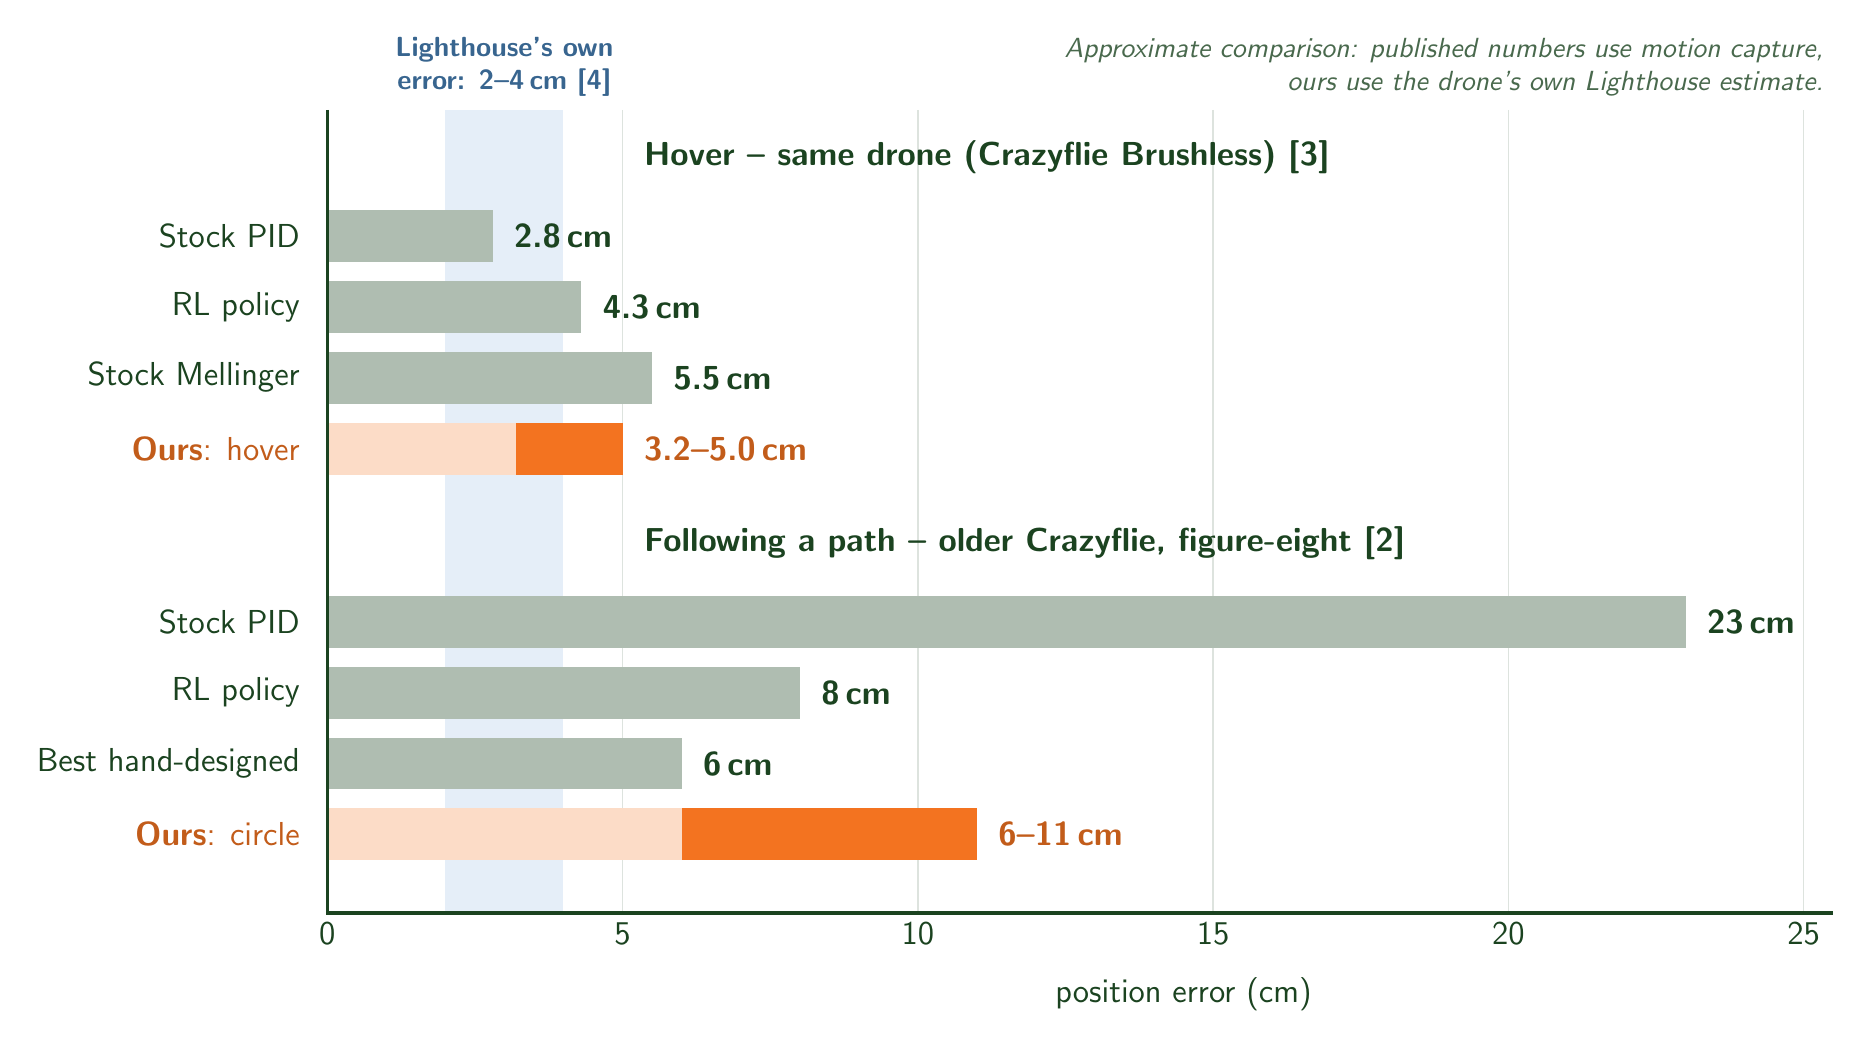
\begin{tikzpicture}[x=0.75cm, y=1cm]
  \def\h{0.33}   % half bar height
  \def\top{1.6}  \def\bot{-8.6}
  % Lighthouse accuracy band
  \fill[bleu!15] (2,\top) rectangle (4,\bot);
  \node[anchor=south, align=center, font=\normalsize\bfseries, text=bleu!70!black] at (3,\top+0.05)
       {Lighthouse's own\\error: 2--4\,cm [4]};

  % grid and axis
  \foreach \x in {0,5,...,25} {
    \draw[saclaydk!15, line width=0.6pt] (\x,\top) -- (\x,\bot);
    \node[anchor=north, font=\large, text=saclaydk] at (\x,\bot) {\x};
  }
  \node[anchor=north, font=\large, text=saclaydk] at (14.5,\bot-0.7) {position error (cm)};

  % group headers
  \node[anchor=west, font=\large\bfseries, text=saclaydk] at (5.2,1.0) {Hover \textendash\ same drone (Crazyflie Brushless) [3]};
  \node[anchor=west, font=\large\bfseries, text=saclaydk] at (5.2,-3.9) {Following a path \textendash\ older Crazyflie, figure-eight [2]};

  % published results (grey bars)
  \foreach \y/\lab/\v in {0/{Stock PID}/2.8, -0.9/{RL policy}/4.3, -1.8/{Stock Mellinger}/5.5,
                          -4.9/{Stock PID}/23, -5.8/{RL policy}/8, -6.7/{Best hand-designed}/6} {
    \fill[saclaydk!35] (0,\y-\h) rectangle (\v,\y+\h);
    \node[anchor=east, font=\large, text=saclaydk] at (-0.3,\y) {\lab};
    \node[anchor=west, font=\large\bfseries, text=saclaydk] at (\v+0.2,\y) {\v\,cm};
  }
  % ours (orange ranges)
  \foreach \y/\lab/\a/\b in {-2.7/{\textbf{Ours}: hover}/3.2/5.0, -7.6/{\textbf{Ours}: circle}/6/11} {
    \fill[mandarine!25] (0,\y-\h) rectangle (\a,\y+\h);
    \fill[mandarine] (\a,\y-\h) rectangle (\b,\y+\h);
    \node[anchor=east, font=\large, text=mandarine!80!black] at (-0.3,\y) {\lab};
    \node[anchor=west, font=\large\bfseries, text=mandarine!80!black] at (\b+0.2,\y) {\a--\b\,cm};
  }
  \draw[saclaydk, line width=1.2pt] (0,\top) -- (0,\bot) -- (25.5,\bot);

  % caveat
  \node[anchor=south east, align=right, font=\normalsize\itshape, text=saclaydk!80] at (25.5,\top+0.05)
       {Approximate comparison: published numbers use motion capture,\\ours use the drone's own Lighthouse estimate.};
\end{tikzpicture}
\end{document}
